
\chapter{Selected Background Information}
\label{ch:selectedBG}

Bioinformatics covers a wide range of scientific fields, such as biology, chemistry and computer science. This chapter gives a short introduction to the areas of bioinformatics relevant to the methods and implementation used in later chapters. 


\section{Proteins}

Proteins play a key role in almost all biological activity. Proteins are large biological polymers composed of one or more chains of amino acids. These amino acids are held together by spatial bonds called peptide bonds. Further information about the material described in this section can be found in \cite{ Nelson.2013, Gromiha.2010, Berg.imp.2002}.

\subsection{Amino Acids}
\label{ssec:AminoAcid}

Amino acids are the basic building blocks of proteins. Each amino acid consists of a central $\alpha$ carbon ($C_\alpha$) bound to:

\begin{itemize}
\item  a carboxyl group ($COOH$)

\item an amino group ($NH_2$)

\item a hydrogen atom ($H$)

\item a distinct side chain (or $R$-group)
\end{itemize}

Variation in the side chain defines the 20 common amino acids found in protein molecules. For instance, if the side chain contains just one hydrogen atom, the amino acid is glycine, while the side chain $CO_2OH$ forms the amino acid serine. Table \ref{tab:AAlist} lists the 20 common amino acids found in proteins with their assigned three-letter abbreviations and one-letter symbols, as defined in \cite{IUPACIUBJointCommissiononBiochemicalNomenclature.1984}. The abbreviations and one-letter symbols are used to simplify computing with amino acid chains.


\begin{table}[h!]
	\centering
	\begin{tabular}{|l|c|c|}
		\firsthline
		Amino acid	  & Abbreviation &
		 One-letter symbol \\ \hline
		Alanine       & Ala  & A   \\
		Arginine      & Arg & R \\
		Asparagine    & Asn & N \\
		Aspartic acid \qquad & Asp & D \\
		Cysteine      & Cys & C \\
		Glutamic acid & Glu & E \\
		Glutamine     & Gln & Q \\
		Glycine       & Gly & G \\
		Histidine     & His & H \\
		Isoleucine    & Ile & I \\
		Leucine       & Leu & L \\
		Lysine        & Lys & K \\
		Methionine    & Met & M \\
		Phenylalanine \quad & Phe & F \\
		Proline       & Pro & P \\
		Serine        & Ser & S \\
		Threonine     & Thr & T \\
		Tryptophan    & Trp & W \\
		Tyrosine      & Tyr & Y \\
		Valine        & Val & V  \\\hline
	\end{tabular}
	\caption[The 20 common amino acids.]{The 20 common amino acids of proteins with their three-letter abbreviations and one-letter symbols \cite{IUPACIUBJointCommissiononBiochemicalNomenclature.1984}.}
 \label{tab:AAlist}
\end{table}


Several additional symbols for so-called ``ambiguous amino acids'' are also defined. These are placeholders for positions in a protein where the exact type of a single amino acid cannot be experimentally determined. For example, the symbol B stands for either aspartic acid or asparagine, while X stands for any one of the 20 common amino acids.






\subsection{Physio-chemical Properties of Amino Acids}
\label{ssec:ppaa}

The side chains of amino acids give them specific properties that influence how each amino acid can interact with its surroundings. 
In \cite{Meiler.2001}, Meiler et al. collected seven unique \acp{PP} for each of the 20 amino acid molecules. These are as follows:



\begin{itemize}
\item \textit{Steric parameter:} The steric parameter is the graph-shape index that characterizes the molecular shape of the molecule through its possible deformations.


\item \textit{Volume:}  The volume is described as the normalized molecular volume occupied by the atoms of an amino acid.

\item \textit{Isoelectric point:} The isoelectric point is the pH-value of a solution in which the amino acid exists in a neutral form, where it is neither positively nor negatively charged. 

\item \textit{Polarizability:} The polarizability is the dynamic response of the molecule to external magnetic fields in order to form instantaneous dipoles. 

\item \textit{Hydrophobicity:}  Hydrophobicity describes the possibility of interactions between polar solvents like water and the side chain of the amino acid. A high hydrophobicity indicates that the residue has a low ability to bind with the solvent.

\item \textit{Helix probability:} This is the probability of an amino acid being identified as $\alpha$-helix in the secondary structure. 

\item \textit{Sheet probability:} This is the probability of an amino acid being identified as $\beta$-sheet in the secondary structure. 

\end{itemize}

The values for these seven \acp{PP} for the 20 amino acids can be found in Appendix \ref{app:PPAA}.



\subsection{Polypeptides}

Two amino acids can form a dipeptide through a covalent chemical bond. This bond is formed through the cleavage of a water molecule ($H_2O$) from the carboxyl group of one amino acid  and the amino group of another. The resulting $CO-NH$ bond is called a \textit{peptide bond} (see Figure \ref{fig:dipeptide}). 

\begin{figure}[b!]
	\begin{center}
		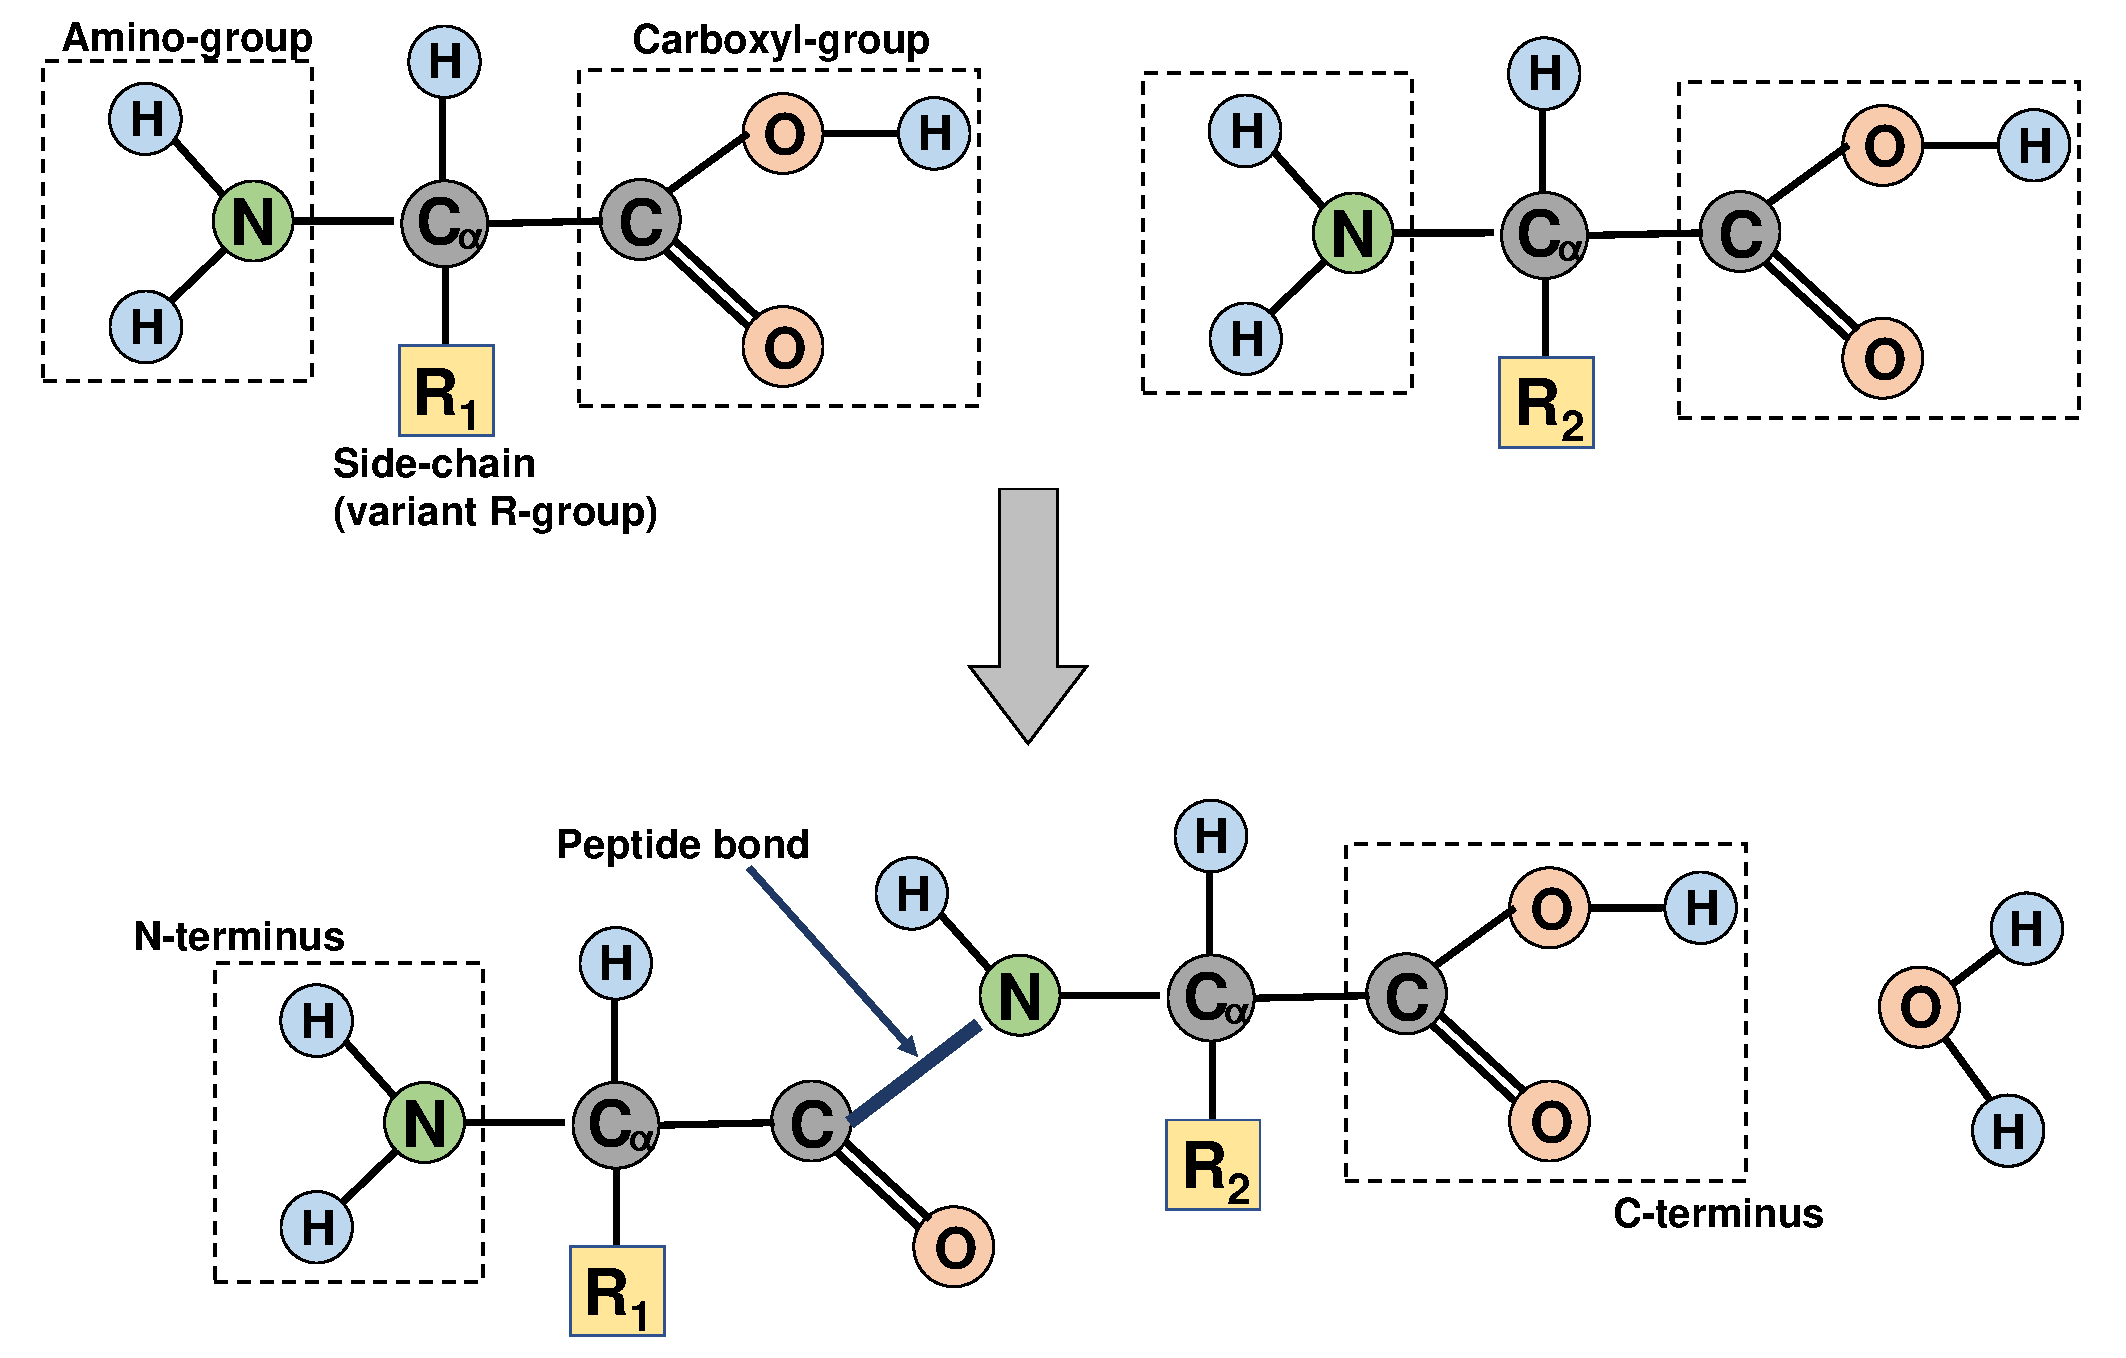
\includegraphics[width=0.94\textwidth]{fig/peptideBond}
	\end{center}
	\caption{Dipeptide forming from the condensation of two amino acids. }
	\label{fig:dipeptide}
\end{figure}

Peptide bonds can extend into peptide chains with a size of up to several thousand  amino acid residues. For example, the longest known and experimentally determined peptide chain is \textit{titin},  with almost 36,000 amino acid residues\footnote{Titin UniProt entry: \url{https://www.uniprot.org/uniparc/UPI000264F4A1} (accessed July 18, 2018).}. However, the average sequence length is 336 amino acid residues\footnote{UniProtKB Statistics: \url{https://www.ebi.ac.uk/uniprot/TrEMBLstats} (accessed July 18, 2018).}.

 By convention, the reading direction of a polypeptide chain is defined from the N- to the C-terminus. The N-terminus refers to the free amino group at one end and the \mbox{C-terminus} to the free carboxyl group at the other end of the chain. 
 Unfolded sequences with up to 50 residues are generally referred to as peptides. For longer sequences, the term ``polypeptide'' is used. 
 One or more polypeptides that together form a biologically functioning unit when folded into a three-dimensional structure are called a protein. 

 



\subsection{Protein Backbone}
\label{ssec:backbone}

The continuous repeated chain of the central covalent bounded atoms \mbox{(-NH-C$_\alpha$-CO-)} in a polypeptide forms the main chain and is referred to as the backbone. 
For each residue in a polypeptide backbone, the three dihedral  angles $\phi$, $\psi$, $\omega$ define its orientation in space. As shown in Figure \ref{fig:dihedral}, the dihedral angle is the torsional angle at the intersection of two planes over four consecutive atoms of the backbone, with the angle $\phi$ between NH and C$_\alpha$, $\psi$  between C$_\alpha$ and CO, and $\omega$ at the peptide bond, from one amino acid residue to the next. 



\begin{figure}[h!]
	\begin{center}
		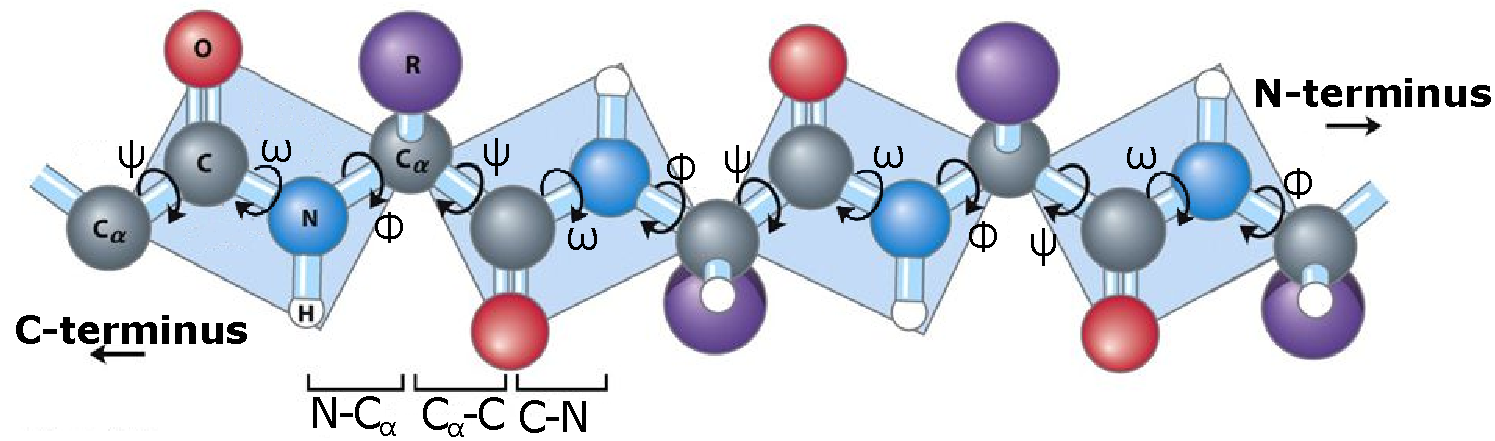
\includegraphics[width=0.8\textwidth]{fig/dihedral}
	\end{center}
	\caption[The dihedral angles $\phi$, $\psi$, $\omega$ in a polypeptide.]{The dihedral angles $\phi$, $\psi$, $\omega$ in a polypeptide, adapted from \cite{Nelson.2013}.}
	
	\label{fig:dihedral}
\end{figure} 

Although the dihedral angles are measured in values from -180$^{\circ}$ to +180$^{\circ}$, the rotation is restricted by several factors.  
Peptide bonds have a partial double-bonded character because they resonate between a single-bond and double-bond state. 
This restricts the rotation angle $\omega$ to two possible configurations, usually with an angle of 180$^{\circ}$ or in some rare cases 0$^{\circ}$. 
The other two angles $\phi$ and $\psi$ are single-bonded and can therefore in principle rotate freely. 
However, the possible orientations are limited by the variant R-group, as atoms of certain side chains may interfere with the backbone. Ramachandran plots are used to display the statistical distribution of the combination of possible conformations for both dihedral angles of each residue.


The Ramachandran plot in Figure \ref{fig:ramachandran} shows the freely available conformation space of amino acid residues, based on the atoms' \textit{van der Waals} radii\footnote{The van der Waals radius is the spherical region of an atom that represents the distance that another atom approaches before the repulsive force becomes too strong.}. 
Green regions mark orientations without interference. The light green regions are less common, especially for residues with larger side chains, but are a possible conformation with reduced van der Waals radii. Except for glycine, white regions are not malleable. Glycine, with its small side chain of just one hydrogen atom, has a broader flexibility and therefore can orient itself in all four quadrants of the Ramachandran plot.

\begin{figure}[h]
	\begin{center}
		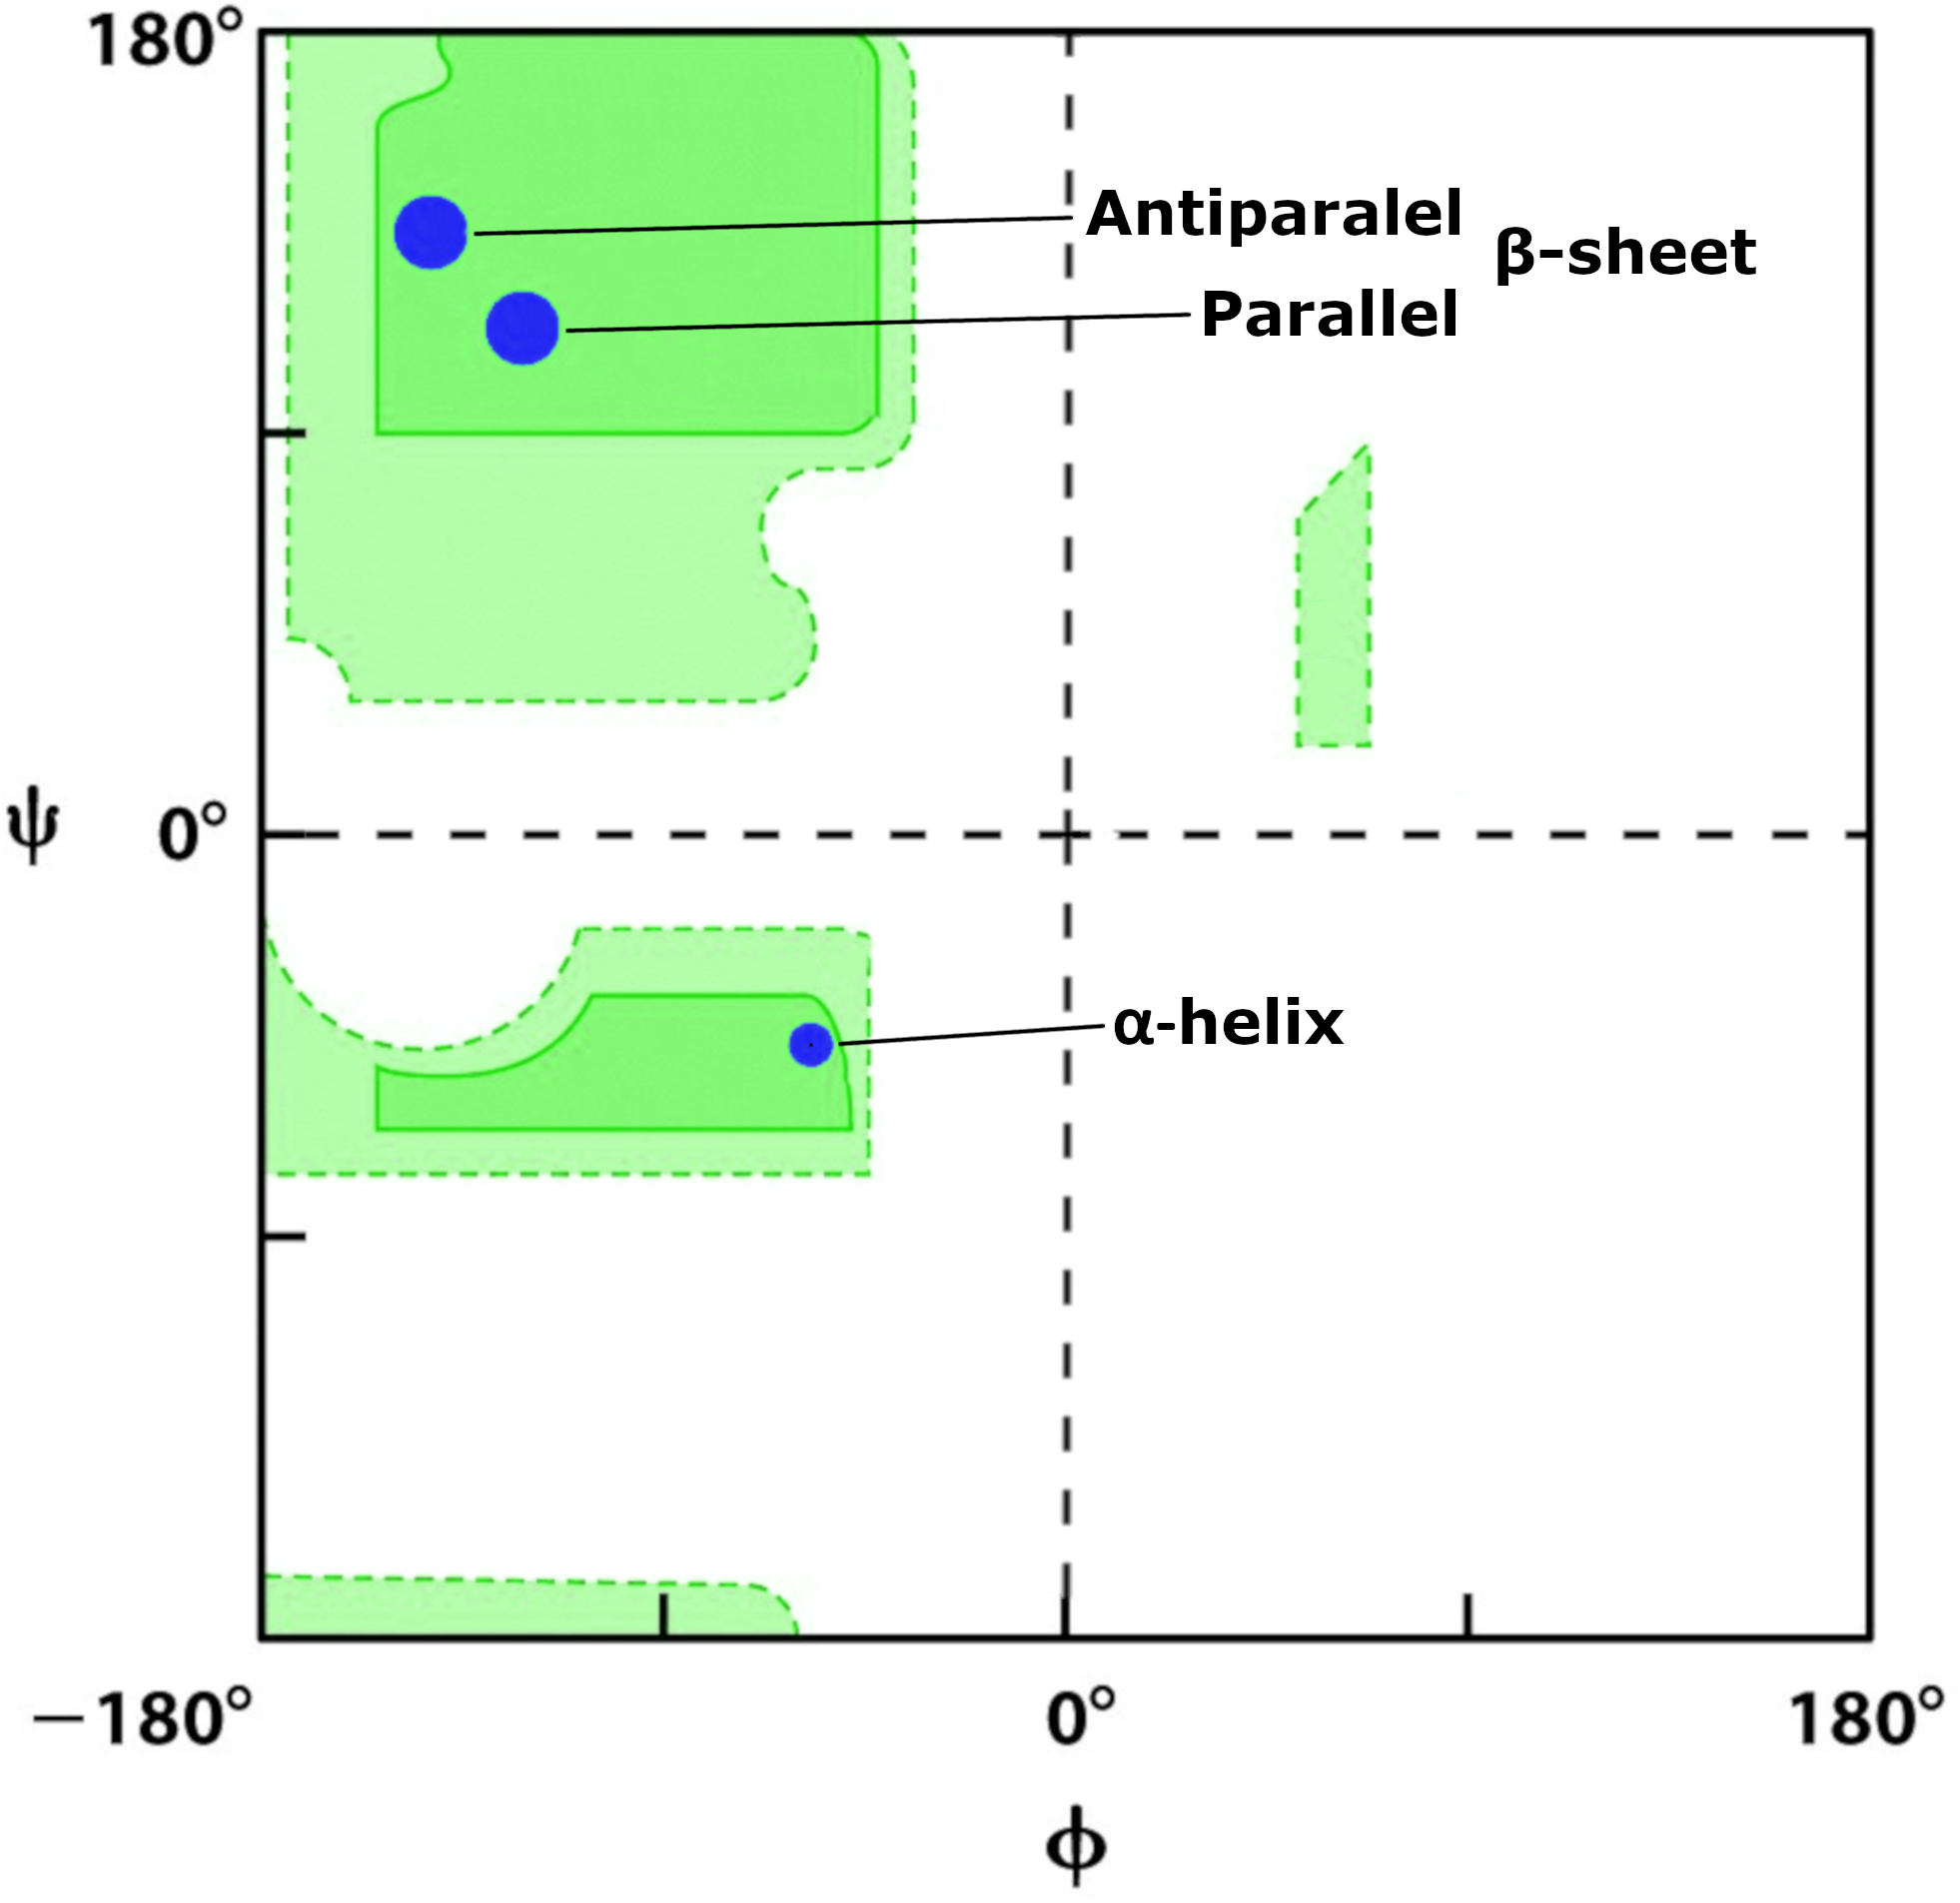
\includegraphics[width=0.54\textwidth]{fig/Ramaplot}
	\end{center}
	
	\caption[Ramachandran plot marking possible conformation of amino acid residues for the dihedral angles.]{Ramachandran plot marking possible conformation of amino acid residues for the dihedral angles $\phi$ on the horizontal and $\psi$ on the vertical axis, adapted from \cite{Nelson.2013}.}
	\label{fig:ramachandran}
\end{figure} 
 
 
% ################################################################
%%----------------------   PROTEIN STRUCTURE    ------------------
% ################################################################
\subsection{Protein Structure}


The shape of a protein is critical to its function. When stretched out, polypeptide chains have no functional activity. They become active when arranged in their stable three-dimensional structure, which is dictated by the chain's amino acid sequence. The protein structure can be divided into four hierarchical levels: primary, secondary, tertiary, and quaternary. These four levels, described in more detail below, are shown in Figure \ref{fig:protein}.

\begin{figure}[h!]
	\begin{center}
		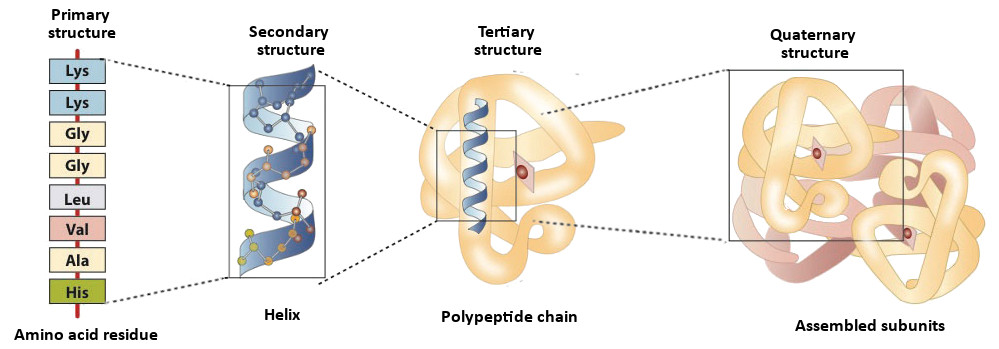
\includegraphics[width=1\textwidth]{fig/BspStruct.jpg}
	\end{center}
	\caption[The four levels of structure in proteins.]{The four levels of structure in proteins \cite{Nelson.2013}.}
	\label{fig:protein}
\end{figure}



The \textbf{primary structure} is represented by the linear sequence of amino acids within a polypeptide connected by peptide bonds, where each element corresponds  to one of the 20 amino acids described in  Section \ref{ssec:AminoAcid}. The primary structure of a polypeptide can  be determined from protein sequencing methods such as spectrometry. 

The \textbf{secondary structure} is defined by the local folding patterns of a region of the protein over a short range of amino acids in a polypeptide. The secondary structure is mainly dependent on the primary structure, which is stabilized by hydrogen bonding due to interaction between the atoms of the backbone.
The two most common spatial formations are the $\alpha$-helix and the $\beta$-sheet, connected by irregular segments referred to as loops or coils. 

The $\alpha$-helix folds by twisting the polypeptide chain into a right-handed coiled structure, with the side chains positioned on the outside of the helix where they are free to interact with the surroundings. The helix is stabilized by hydrogen bonds between the oxygen of the carboxyl group from one residue and the hydrogen from the amino group of the fourth-next amino acid residue in the polypeptide chain.
 Each full turn of the helix contains 3.6 amino acid residues. For all amino acids in an $\alpha$-helix formation, both dihedral angles $\phi$  and $\psi$ are negative, with regions around of -57$^{\circ}$ and -47$^{\circ}$, respectively, as marked in the third quadrant of the Ramachandran plot in Figure \ref{fig:ramachandran}.

The $\beta$-sheet is composed of two or more stretched polypeptide segments, also called $\beta$-strands, which are positioned next to each other and held together by hydrogen bonds. The side chains in $\beta$-sheets alternate above and below the plane of the strands.  Due to the direction of polypeptides, $\beta$-sheets can be differentiated into anti-parallel $\beta$-sheets when the strands run in opposite directions and parallel $\beta$-sheets when they run in the same direction. In the Ramachandran plot, the $\beta$-sheet is located in the second quadrant with a positive $\phi$ and negative $\psi$   of around  -139$^{\circ}$ and +135$^{\circ}$, respectively, for parallel $\beta$-sheets, and with -119$^{\circ}$ and 113$^{\circ}$, respectively, for anti-parallel $\beta$-sheets. 

Loops or coils are irregular regions of a polypeptide not recognized as one of the two above, and mainly connect these other structures. However, some patterns are distinguishable, for example hairpin loops between  two anti-parallel $\beta$-sheets that can be as short as two residues. Turns are narrow 180$^{\circ}$ loops.

If the tertiary structure is available, the secondary structure can (almost trivially) be computed from the former. Otherwise, it has to be predicted from the primary structure. Methods for secondary structure determination are explained in Section \ref{ssec:SSPred}.


The \textbf{tertiary structure} is defined by the coordinates of all the atoms in the protein relative to one another and represents the complete three-dimensional structure of the entire folded polypeptide chain. Beside hydrogen bonds, the tertiary structure is also stabilized by ionic bonds, van der Waals interactions and disulfide bridges. 
Ionic bonds form between oppositely charged amino acid side chains, such as lysine with aspartic acid.
A van der Waals interaction is a weak force of attraction between adjacent atoms that come close to their outer electron cloud, which induces charge fluctuations. Disulfide bonds are like peptide bonds. They are covalent bonds, but they form between the side chains of two \textit{cysteine} amino acids.
The tertiary structure of a protein is determined by experimental methods such as \ac{XRC}  and \ac{NMR} spectroscopy. 


The \textbf{quaternary structure} represents complex protein structures made up of multiple polypeptide chains and shows how they interact with one another. For example, hemoglobin is made up of four polypeptide chains. Linked together, they serve functions such as oxygen and carbon dioxide transport in red blood cells.




\subsection{Protein Folding}

Peptide chains are assembled piece by piece from the synthesis of \ac{RNA} molecules. These \ac{RNA} molecules contain the blueprint of the amino acid sequence given from the genetic code in the \ac{DNA}. 
These sequences are built without a specific shape as unfolded chains or random coils. Protein folding is the process in which the unstable chain is translated into its native three-dimensional structure in order to function correctly.  
The three-dimensional conformation is influenced by several factors, in particular forces from the interaction of the atoms in the side chains and the thermodynamics of the structure. 
During the synthesis, short local conformations such as helices and strands begin to form. Subsequently, the whole sequence begins to move until it reaches its native shape, which requires the lowest energy conformation to stay in shape.  
However, folded proteins are still flexible to a certain degree, as their functional properties may require a dynamic structure. 
One of the biggest challenges in bioinformatics in recent decades has been the protein-folding problem, which tries to fully understand the dynamics and mechanics of the folding process in order to predict the native structure of a protein from its amino acid sequence. 
 Although the folding process of some peptides can already be predicted with reasonable accuracy, understanding the complete process remains an unresolved problem. Improving our knowledge of the folding process is important to treat diseases caused by misfolding  \cite{Dill.2012}.

Misfolding of proteins is one of the main causes of many different types of diseases, such as cancer, Alzheimer’s and Parkinson’s. Mutations in the DNA cause changes in the amino acid composition during the synthesis, which changes the three-dimensional shape of a protein and thus influences the function of the protein. An example in which a small change in amino acid composition has a significant impact on the fold is sickle cell disease, where in one of the peptide chains of hemoglobin, the amino acid valine is placed at the sixth position of the chain instead of glutamic acid. This mutation causes a deformation of the red blood cells from a disc shape to a sickle-shaped structure. This reduces the cells’ ability to transport oxygen through the body. The lack of oxygen transport can lead to symptoms such as anemia and bacterial infections and in the long term can cause death.
 


\subsection{Protein Functions}

Proteins are central elements in all living organisms. They serve many different functions in the body and can be described mainly in terms of the following functional tasks:

\begin{itemize}

\item \textit{Enzyme}: Enzymes are catalysts that are responsible for carrying out all biochemical reactions that take place in body cells. For example, \textit{pepsin} is an enzyme protein in the stomach that is responsible for digesting other proteins in food.

\item \textit{Messenger}: Messenger proteins, such as most hormones, are responsible for the communication of cells in one part of the body with cells in another part of the body to coordinate biological processes between different parts of the body. Messenger proteins are generally relatively small peptides. For example, \textit{insulin}, with 51 amino acid residues, regulates the metabolism of carbohydrates and fats.


\item \textit{Structural Protein:}
Structural proteins maintain the structural integrity of cells, organs and connective tissues and are sometimes involved in cell movement. An example is \textit{keratin}, which serves as a protective cover of many different body parts, such as skin, hair and nails.

\item \textit{Transport:}
Carrier molecules or transport proteins are responsible for carrying and sometimes also storing substances within the body. For example, \textit{hemoglobin} takes oxygen from the lungs and transports it in the blood through the body to the tissues. Other transport proteins include \textit{myoglobin}, which takes the oxygen from the hemoglobin and stores it until needed by the muscle tissue.


\item \textit{Antibody:}
Antibodies are proteins in the blood that defend the body against diseases from harmful intruders such as viruses or bacteria. When intruders enter the body, the immune system creates antibodies to identify the intruders in the body and destroy them.

\end{itemize}
 

\subsection{Protein Homology}

Two proteins are homologous when they share common evolutionary ancestors. 
Often, homologous proteins with similar biological functions have similar sequences and structures, at least in some crucial regions. Differences occur due to mutations in the sequence, such as substitutions, insertions, and deletions of single amino acids. 
The degree of homology is determined by metrics such as the similarity of two sequences. 
High sequence similarity between two sequences is an indication of a shared ancestor, whereas the probability of these sequences having originated independently of each other increases with decreased sequence similarity. As the structural fold of a protein is crucial to its function, regions that are critical to its function are more conserved than irregular loops.
A way to model and describe  protein homology is to use \acp{MSA} (see Section \ref{sec:MSA}). 

